\documentclass{llncs}
\pagestyle{plain}
%\usepackage[margin=2.5cm]{geometry}
\usepackage[pdftex]{graphicx}
\usepackage{caption}
\usepackage{subcaption}
\usepackage[rightcaption]{sidecap}
\usepackage{float}
\usepackage[ruled, vlined, linesnumbered]{algorithm2e}
\SetAlgoSkip{bigskip}
\usepackage{hyperref}
\usepackage{amsmath}
\usepackage{titling}
\usepackage{soul}
\usepackage{cite}

\usepackage{fancyhdr}
\pagestyle{fancy}
\fancyhf{}
\lhead{Swarm Intelligence}
\rhead{Winter 2014/15}
\cfoot{\thepage}

\setlength{\droptitle}{-4em}
\title{Collective Decision Making with Heterogeneous Agents}
\author{Syam Ajay Simha Gullipalli\\
		Universit\"at Paderborn\\
		\texttt{syam@mail.uni-paderborn.de}}
\date{\today}

\begin{document}
	\maketitle
	\thispagestyle{fancy}
	
	\section{Introduction} \label{sec:introduction}

	
	\section{State Machine}	
	
	%FIGURE: Image Graph
	\begin{figure}
		\centering
		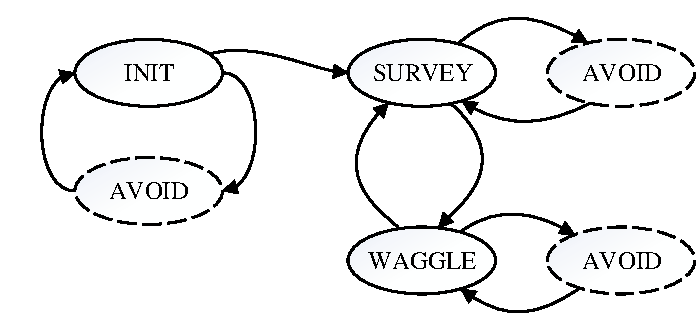
\includegraphics[width=0.7\textwidth]{IMG/StateMachine}
		\caption{State machine for collective decision making using house hunting behavior of honeybees and  opinion dynamics.}
		\label{fig:stateMachine}
	\end{figure}
	
	
	\begin{equation}
		\centering
		\tau^{n}_{ij} \leftarrow (1 - \rho) \cdot \tau_{ij} + \rho \cdot \Delta \tau^{k}_{ij}
		\label{eq:globalupdate}
	\end{equation}
	
	
	
	%Comparision
	\section{Results}\label{sec:comparision}

	
	
	
	
	%Conclusion
	\section{Conclusion}\label{sec:conclusion}
	
	
	
	\bibliographystyle{splncs}
	\bibliography{literature}
	\nocite{*}
	
\end{document}